\chapter{Hyperparameters}
\label{app:hyperparameters}

\begin{table}
    \centering
    \begin{tabular}{c|ccc}
        \textbf{Dataset} &
        \textbf{Layers} &
        \textbf{Learning rate} &
        \textbf{Epochs} \\
        \midrule
        BA Shapes       & 3 $\times$ 20 & 0.001 & 3000 \\
        BA Grid         & 3 $\times$ 20 & 0.001 & 3000 \\
        BA Community    & 6 $\times$ 50 & 0.001 & 6000 \\
        Tree Cycles     & 3 $\times$ 50 & 0.001 & 7000 \\
        Tree Grid       & 7 $\times$ 20 & 0.001 & 10000 \\
        \midrule \\
        REDDIT BINARY   & 4 $\times$ 40 & 0.005 & 3000 \\
        Mutagenicity    & 4 $\times$ 30 & 0.005 & 10000 \\
    \end{tabular}
    \caption{GCN hyperparameters from table 15 in \textit{Magister et al.}\cite{magister2021gcexplainer}. All models use \texttt{ReLU}\note{citation needed?} activation functions between layers with a single linear layer classifier with \texttt{softmax}\note{citation needed?}.}
    \label{tab:GCN-params}
\end{table}


\begin{table}[h]
    \centering
    \captionsetup{width=.9\textwidth}
    \begin{tabular}{c|cccc}
        \textbf{Dataset} &
        \textbf{Degree} &
        \textbf{Learning rate} &
        \textbf{Weight decay} &
        \textbf{Epochs} \\
        \midrule
        Cora        & 2 & 0.002 & 0.04 & 100 \\
        Citeseer    & 2 & 0.004 & 0.08 & 100 \\
        PubMed      & 2 & 0.0005 & 0.25 & 100 \\
    \end{tabular}
    \caption{SGC hyperparameters using \texttt{hyperopt}\cite{bergstra2013making} as proposed by \textit{Wu et al.}\cite{wu2019simplifying}. All models use \texttt{softmax}.}
    \label{tab:SGC-reproduction-params}
\end{table}


\begin{table}
    \centering
    \begin{tabular}{c|cccc}
        \textbf{Dataset} &
        \textbf{Degree} &
        \textbf{Learning rate} &
        \textbf{Weight decay} &
        \textbf{Epochs} \\
        \midrule
        BA Shapes       & 3 & 0.01 & 0.1 & 3000 \\
        BA Grid         & 3 & 0.01 & 0.1 & 3000 \\
        BA Community    & 6 & 0.001 & 0.1 & 6000 \\
        Tree Cycles     & 3 & 0.01 & 1.0 & 7000 \\
        Tree Grid       & 7 & 0.01 & 0.01 & 10000 \\
    \end{tabular}
    \caption{SGC hyperparameters based on the corresponding GCN hyperparameters in \ref{tab:GCN-params} and using the results of the hyperparameter search in \note{reference when added}. All models use \texttt{softmax}\note{citation needed?}.}
    \label{tab:SGC-params}
\end{table}


\begin{table}[h]
    \centering
    \captionsetup{width=.9\textwidth}
    \begin{tabular}{c|cccc}
        \textbf{Dataset} &
        \textbf{Degree} &
        \textbf{Learning rate} &
        \textbf{Weight decay} &
        \textbf{Epochs} \\
        \midrule
        BA Shapes       & 3 & 0.001 & 0.01 & 1200 \\
        BA Community    & 6 & 0.001 & 0.01 & 1400 \\
    \end{tabular}
    \caption{JSGC hyperparameters based on the corresponding SGC hyperparameters in \ref{tab:SGC-params} and using the results of the hyperparameter searchs in figure \ref{fig:JSGC-surfaces}. All models use \texttt{softmax} and \texttt{ReLU} between the aggregation of jumping knowledge and the classifier.}
    \label{tab:JSGC-params}
\end{table}


\begin{table}[h]
    \centering
    \captionsetup{width=.9\textwidth}
    \begin{tabular}{c|cc}
        \textbf{Dataset} &
        \textbf{Clusters (k)} &
        \textbf{Receptive field (n)} \\
        \midrule
        BA Shapes       & 10 & 2 \\
        BA Grid         & 10 & 3 \\
        BA Community    & 30 & 2 \\
        Tree Cycles     & 10 & 3 \\
        Tree Grid       & 10 & 3 \\
        \midrule
        REDDIT BINARY   & 20 & 1 \\
        Mutagenicity    & 30 & 3 \\
    \end{tabular}
    \caption{Concept extraction parameters used in \textit{Magister et al.}\cite{magister2021gcexplainer}.}
    \label{tab:GCN-concept-params}
\end{table}



\begin{figure}
    \centering
    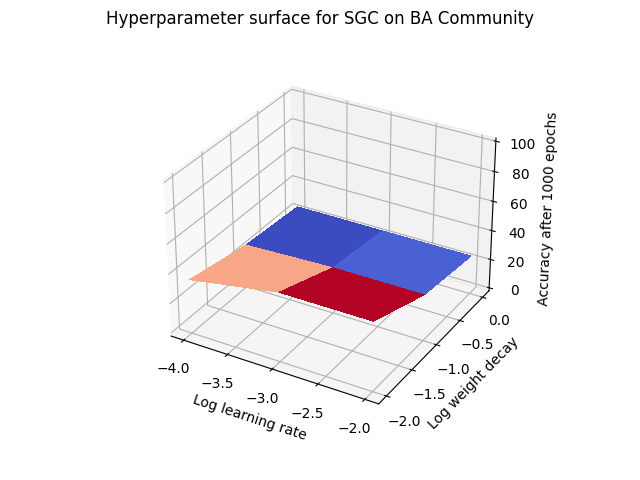
\includegraphics[width=0.45\textwidth]{figures/SGC-BA-Community-surface}
    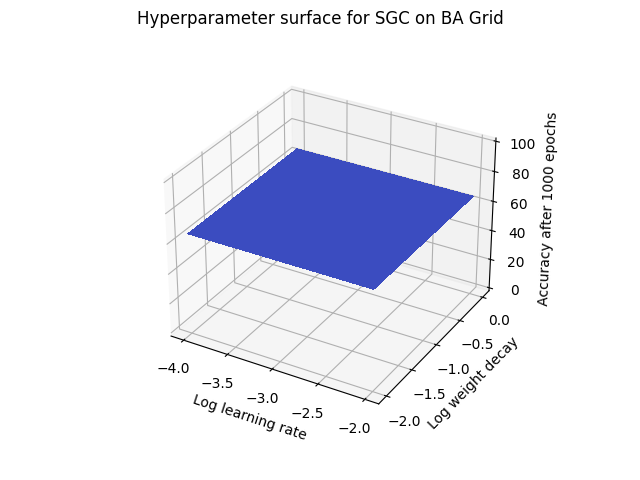
\includegraphics[width=0.45\textwidth]{figures/SGC-BA-Grid-surface}
    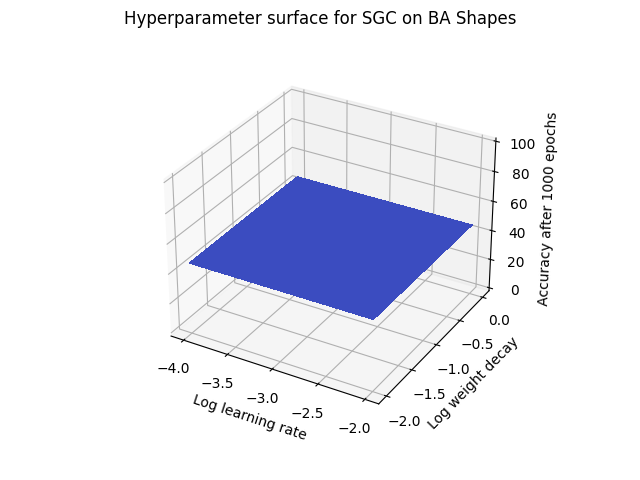
\includegraphics[width=0.45\textwidth]{figures/SGC-BA-Shapes-surface}
    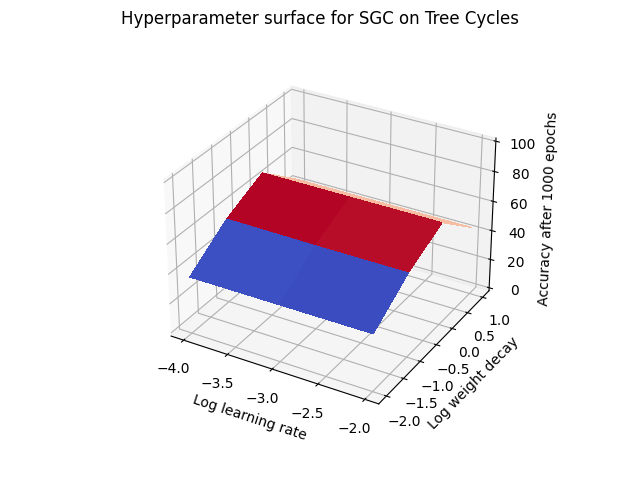
\includegraphics[width=0.45\textwidth]{figures/SGC-Tree-Cycles-surface}
    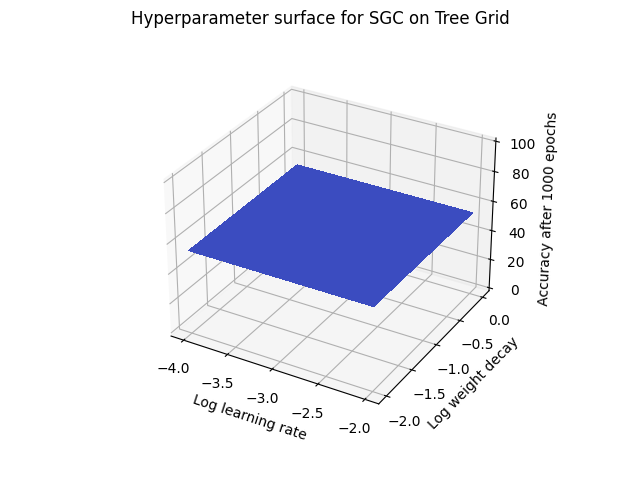
\includegraphics[width=0.45\textwidth]{figures/SGC-Tree-Grid-surface}
    \caption{SGC hyperparameter surfaces for learning rates in $\{0.01, 0.001, 0.0001\}$ and weight decay constants in $\{1, 0.1, 0.01\}$. In the case of Tree Cycles enough of an improvement is seen to warrant the additional weight decay constant $10$.}
    \label{fig:SGC-surfaces}
\end{figure}

\begin{figure}
    \centering
    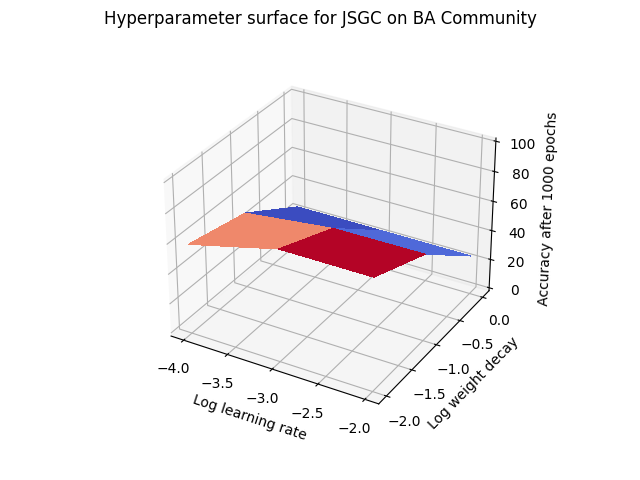
\includegraphics[width=0.45\textwidth]{figures/JSGC-BA-Community-surface}
    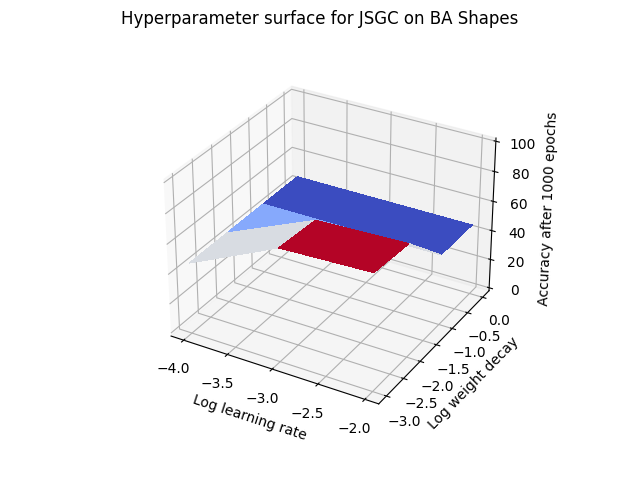
\includegraphics[width=0.45\textwidth]{figures/JSGC-BA-Shapes-surface}
    \caption{JSGC hyperparameter surfaces for learning rates in $\{0.01, 0.001, 0.0001\}$ and weight decay constants in $\{1, 0.1, 0.01\}$. In the case of BA Shapes enough of an improvement is seen to warrant the additional weight decay constant $10$.}
    \label{fig:JSGC-surfaces}
\end{figure}

